%%%%%%%%%%%%%%%%%%%%%%%%%%%%%%%%%%%%%%%%%%%%%%%%%%%%%%%%%%%%%%%%%%%%%%%%%%%%%%%%%%%%%%%%%%%%%%%%%%%
% Chapter 4 -> MOJITOO Experiments and Results
% Author: Mingbo Cheng
%%%%%%%%%%%%%%%%%%%%%%%%%%%%%%%%%%%%%%%%%%%%%%%%%%%%%%%%%%%%%%%%%%%%%%%%%%%%%%%%%%%%%%%%%%%%%%%%%%%
%\addbibresource{~/MEGA/MEGAsync/phd/thesis_Cheng/preamble/thesis.bib}
\chapter{MOJITOO Experiments \& Results }
\label{chapter:MOJITOO_bench}

\graphicspath{{chapter4/figs}}
In the previous chapter, we introduced our computational approach, MOJITOO, for the integration of single-cell multimodal data. Here, we outline the experimental framework employed in this thesis to validate our method and subsequently present the results. The framework comprises two sections: technical validation and biological validation. In technical validation (Section 4.1.1), the primary objective is to assess the performance of our approach and compare it to other methods. Moving to biological validation (Section 4.1.2), we apply MOJITOO to the \texttt{PBMC-Multiome} data generated from mouse Peripheral Blood Mononuclear Cells(PBMC). We test its capability to integrate each canonical component (CC) of the data and its effectiveness in identifying top genes and peaks associated with each CC to gain insights into the data.

In Section 4.2, we present the results described in Section 4.1. Specifically, in 4.2.1, we showcase the technical validation by comparing clustering accuracy, distance accuracy, and structure preservation among competing methods. Additionally, we provide a comparison of computational resources, highlighting the efficiency of these methods. Next, we will introduce (in Section 4.2.2) the biological validation to demonstrate the effectiveness of MOJITOO in PBMC data. We conclude this chapter with a final discussion of our experimental workflow and the results in Section 4.3.


\section{Experiments}
\label{MOJITOO:exp}
In this section, we outline the experimental framework. We begin by introducing the single-cell multimodal data used in the benchmarking (Section 4.1.1). Following that, we delve into the specifics of executing eight computational single-cell integration approaches (Section 4.1.2). Subsequently, we present the technical evaluation of the competing methods (Section 4.1.3). Moving on, we showcase the biological inspection (Section 4.1.4). Finally, we provide a list of the statistical methods employed (Section 4.1.5).

\subsection{Multimodal benchmarking data}
\label{MOJITOO:exp:data}
We utilize publicly available multimodal datasets with two or three modalities in our evaluation. The initial two datasets consist of single-cell CITE-seq data, capturing single-cell RNA and surface proteins simultaneously. The third and fourth datasets involve single-cell data measuring both single-cell RNA and single-cell ATAC simultaneously. Lastly, the last two datasets encompass single-cell data that simultaneously measure single RNA, single-cell ATAC-seq, and single-cell protein. \tref{tab:MOJITOO_DATA} summarize the detail of these data.

\begin{table}[!ht]
	\footnotesize
	\centering
	\begin{tabular}{lllllrrp{0.15\linewidth}}
		\toprule
		{\textbf{Dataset}} & {\textbf{Protocol}} & {\textbf{Species}}  &{\textbf{Organ}}  & {\textbf{Modalities}} &{\textbf{\#cells}}  &{\textbf{\#Cell types}}   &{\textbf{\#Features (gene/peak/protein)}} \\ 
		\midrule
		  BM-CITE  & CITE-seq & Human & Bone Marrow & RNA/protein & 30,672  & 27 & 17,009/-/25 \\
		  LUNG-CITE  & CITE-seq & Human & PBMC\&Lung & RNA/protein & 10,470  & 22 & 33,514/-/52 \\
		  PBMC-Multiome  & Multiome & Human  & PBMC & RNA/ATAC & 11,787 & 13 & 36,610/108,377/- \\ 
		  Skin-SHARE  & SHARE-seq & Mouse & Skin & RNA/ATAC & 34,774 & 23 & 23,296/344,592/- \\ 
		  PBMC-TEA  & TEA-seq  & Human & PBMC & RNA/ATAC/epitope & 25,517 & 12 &  36,601/128,853/47\\ 
		  PBMC-DOGMA  & DOGMA-seq & Human & PBMC & RNA/ATAC/protein & 13,763  & 27 & 36,495/68,963/210 \\
		\bottomrule
	\end{tabular}
	\vspace{0.1cm}
	\caption[Major characteristics of multi-modal data sets]{Major characteristics of multi-modal data sets.}
	\label{tab:MOJITOO_DATA}
\end{table}


\begin{description}
	\item[{\texttt{BM-CITE}}]
	The human bone marrow mononuclear cells ({\texttt{BM-CITE}}) data set contains full transcriptomes and 25 surface proteins for over 30,672 cells annotated in 27 cell types~\citep{hao2021seurat4}. This data was obtained with the ``LoadData("bmcite")'' command from the package SeuratData. 

	\item[{\texttt{LUNG-CITE}}]
	The \texttt{LUNG-CITE} is derived from CITE-seq protocol which uses the human peripheral blood mononuclear cells from the lung ({\texttt{LUNG-CITE}}) ~\citep{buus2021improving} with 52 surface proteins. It contains 10,470 cells annotated in 22 cell types. This data was obtained from ~\url{https://tinyurl.com/253jp4sa}.

	\item[{\texttt{PBMC-multiome}}]
  	The data set contains human peripheral blood mononuclear cells ({\texttt{PBMC-multiome}}) generated by the 10x multiome technology to measure gene expression (scRNA-seq) and chromatin accessibility (scATAC-seq) on the same cells. This data contains 11,787 cells with 13 cell types annotated by 10X Genomics.  We use the scRNA-seq and scATAC-seq count matrices as provided by 10x genomics after processing with the Cellranger pipeline obtained from the ~\url{https://tinyurl.com/yw229pbf}.

	\item[{\texttt{PBMC-multiome}}]
	The data set is based on the SHARE-seq protocol measuring gene expression and chromatin accessibility of mouse skin cells ({\texttt{ SKIN-SHARE}})~\citep{ma2020chromatin}. This data contains 34,774 cells, which are annotated as 23 cell types. We obtain the skin scRNA-seq and scATAC-seq counts and fragments files from the Gene Expression Omnibus under accession number (\href{https://www.ncbi.nlm.nih.gov/geo/query/acc.cgi?acc=GSE140203}{GSE140203}).

	\item[{\texttt{PBMC-DOGMA}}]
	This tri-modal data set of human PBMCs is measured with the DOGMA-seq protocol~\citep{mimitou2021scalable}. This provides RNA, ATAC and epitope sequencing of the same cells ({\texttt{PBMC-DOGMA}}). We use data under low-loss lysis conditions containing 13,763 cells in 27 cell types. We download count matrices as provided by the authors ~\url{https://osf.io/6kr4v/}.

	\item[{\texttt{PBMC-TEA}}]
	The tri-modal dataset is based on human PBMCs measured with the TEA-seq protocol~\citep{swanson2021simultaneous}. It contains transcripts, epitopes and chromatin accessibility of 25,517 PBMCs grouped into 12 cell types ({\texttt{PBMC-TEA}}). For this data set, we obtain original matrices and combine data from distinct wells from GEO (GSE158013). As this scATAC-seq lacks uniform peaks, we create an integrated matrix by combining peaks, allowing an extension of 250 bps. Ultimately, we intersect all barcodes from scRNA-seq, protein, and scATAC-seq to obtain matrices in the same cellular space.
\end{description}

\subsection{Execution of single cell multi-modal integration data}
\label{MOJITOO:exp:run}
% List how to install and run the competing methods

\subsubsection{Preprocessing}
\label{MOJITOO:exp:preprocessing}
We initiate a standardized pre-processing pipeline for all previous datasets, commencing from their count matrices. The specifics of the pre-processing steps for individual modality data are outlined, with additional steps described for a dataset requiring batch correction.
\begin{description}
    \item[scRNA-seq data]
    We follow the standard Seurat 4 pipeline (\href{https://satijalab.org/seurat/articles/pbmc3k_tutorial.html}{source}). Initially, we log normalize the data using the NormalizeData function with default parameters. Subsequently, we identify the top 3000 variable features through FindVariableFeatures and perform data scaling using ScaleData. Finally, we employ RunPCA to conduct dimension reduction~\citep{hao2021integrated}, retaining the first 50 principal components.
    
    \item[scATAC-seq data]
    We adhere to the standard pipeline outlined in the \href{https://satijalab.org/signac/articles/pbmc_vignette.html}{Signac} documentation~\citep{signac}. This involves applying TF-IDF (term frequency-inverse document frequency) on the peaks, running RunSVD on the top features obtained from the FindTopFeatures function with min.cutoff=`q0' parameter, resulting in an LSI dimension-reduced matrix. We retain the first 50 dimensions, excluding the first dimension due to its high correlation with the number of fragments.  
    
    \item[Protein data]
    We adopt the standard Seurat 4 \href{https://satijalab.org/seurat/articles/multimodal_vignette.html}{pipeline}\citep{hao2021integrated}. In summary, we use NormalizeData with parameters normalization.method = `CLR' and margin = 2, followed by ScaleData and RunPCA with 30 PCs using default parameters.
    
    \item[Additional step] 
    \texttt{PBMC-DOGMA} is the only data set evaluated here with two biological conditions (stimulated and unstimulated). To address the presence of batch, we employ Harmony integration\citep{korsunsky2019harmony} independently for RNA-seq and epitope data, integrating control and stimulated samples. For scATAC-seq, integration is carried out by disregarding the first LSI dimension, highly correlated with the stimulation. \afref{fig:batch_correction} illustrates MOJITOO results both with and without batch correction.
\end{description}

\subsubsection{Competing methods}
\label{MOJITOO:exp:methods}
%% TODO: need split these into two parts: algorithm(chapter2) and execution(chapter).
Here, we describe the installation and execution procedures for the competing methods.
\begin{description}
    \item[MOFA] 
    We obtained MOFA2 (version 1.2.2)\citep{tewari2017mofa} from \href{https://github.com/bioFAM/MOFA2}{https://github.com/bioFAM/MOFA2} and installed it using the command `R CMD INSTALL MOFA2'. Subsequently, we executed MOFA with default parameters and followed their recommendations in the tutorial \url{https://raw.githack.com/bioFAM/MOFA2_tutorials/master/R_tutorials/10x_scRNA_scATAC.html} for analyzing all the data. However, we now provide PCA/LSI reductions as input for MOFA, as this has improved its computational time (Appendix ~\atref{tab:time}), as well as the clustering performance in MOFA's latent space\afref{fig:MOFA}.
    
    \item[Schema]
    We installed Schema (version 0.1.5.3)~\cite{singh2021schema} using the command `pip install schema\_learn' in the python==3.9.6 environment. Schema has its exclusive pre-processing and dimension reduction steps, so we retained these steps for multimodal data and performed the integration with default parameters as per their tutorial available at \url{https://schema-multimodal.readthedocs.io/en/latest/recipes/index.html}.
    
    \item[Seurat4 WNN]
    We installed Seurat (version 4.3.0) using `remotes::install\_version(``Seurat", version = ``4.3.0")' in the R (version 4.1.0) prompt. Subsequently, we executed WNN, an integral part of Seurat 4, using default parameters. 
    
    \item[scAI]
    We installed scAI(1.0.0) using `devtools::install\_github(``sqjin/scAI'')' in the R prompt. We execute scAI in only bi-modal with RNA and ATAC-seq datasets with default parameters according to their tutorial example \url{https://htmlpreview.github.io/?https://github.com/sqjin/scAI/blob/master/examples/walkthrough_simulation.html}.
    
    \item[LIGER]
    We install LIGER~\cite{kriebel2021nonnegative} new version rliger(1.0.0) using `R install.packages(``rliger'')' in the R prompt. LIGER~\cite{kriebel2021nonnegative} can perform integration, whenever there is some overlap between the features across modalities (shared features), i.e. protein and RNA expression of the same gene or gene accessibility scores for ATAC-seq. LIGER estimates a gene accessibility (ATAC-seq) matrix by counting the total number of ATAC-seq reads within the gene body and promoter regions(3kb upstream) for each gene per cell. An additional unshared feature matrix is further produced by binning the genome into bins of 100,000 bps and counting the overlap of these bins with peaks from the respective data set. Regions associated with ENCODE Blacklist regions~\cite{amemiya2019encode} are removed, see in detail\citep{liu2020jointly}. To note, LIGER can be only executed for bi-modal data sets. We run LIGER according to their tutorial \url{http://htmlpreview.github.io/?https://github.com/welch-lab/liger/blob/master/vignettes/UINMF_vignette.html}. Since LIGER only provides latent spaces for each modality without a unified space, we simply combine the dimensions from the two modalities to obtain a shared space.
    
    \item[Symphony Integration]
    The CCA analysis is not part of Symphony~\cite{kang2021symphony} source code, we implemented it based on a script provided by authors (\url{https://github.com/immunogenomics/TB_Tcell_CITEseq/blob/main/R/cca_analysis.R}). Also, due to high computational requirements, we were only able to run this on the dimension-reduced space (PCA/LSI) described above. We call this method Symph-Int to reflect the fact that this is not Symphony, but an integration method used in one of the analyses of Symphony manuscript. 
    
    \item[DIABLO]
    We installed mixOmics (version 6.16.3), which includes the implementation of DIABLO~\cite{singh2019diablo}, using Bioconductor with the command BiocManager::install("mixOmics") in the R prompt. DIABLO integrates multiple data sets in a supervised way and was originally designed for bulk multi-omics data, where sample labels are available and explored for feature selection. Since labels are not available for the single-cell multi-modal data evaluated here, we provide a distinct label for each cell. DIABLO is executed as indicated in their tutorial \url{{http://mixomics.org/mixdiablo/}}. Due to prohibitive computational costs if raw matrices are used, we provide dimension-reduced matrices as input. Another major parameter is the number of CC components, which is usually set to the number of classes minus 1, but this is too large for single-cell data. Here, we used 30 components. Additionally, DIABLO does not provide a common latent space. Therefore, we used the same strategy to combine latent spaces as for MOJITOO.
\end{description}

\subsection{Evaluation of multi-modal integration Methods}
\label{MOJITOO:exp:metrics}
In this section, we outline the methodology employed to assess the results generated by executing the single-cell multimodal integration methods, as described earlier.


We employed various metrics to evaluate the single cell mulitmodal integration methods, including structure preservation, distance accuracy, clustering accuracy, and computational resource requirements, such as memory usage and running time consumption. These metrics allowed us to assess the results from different perspectives. \fref{fig:evaluation_MOJITOO} provides an overview framework for the integration methods' evaluation.
\begin{figure}[!ht]
	\centering
	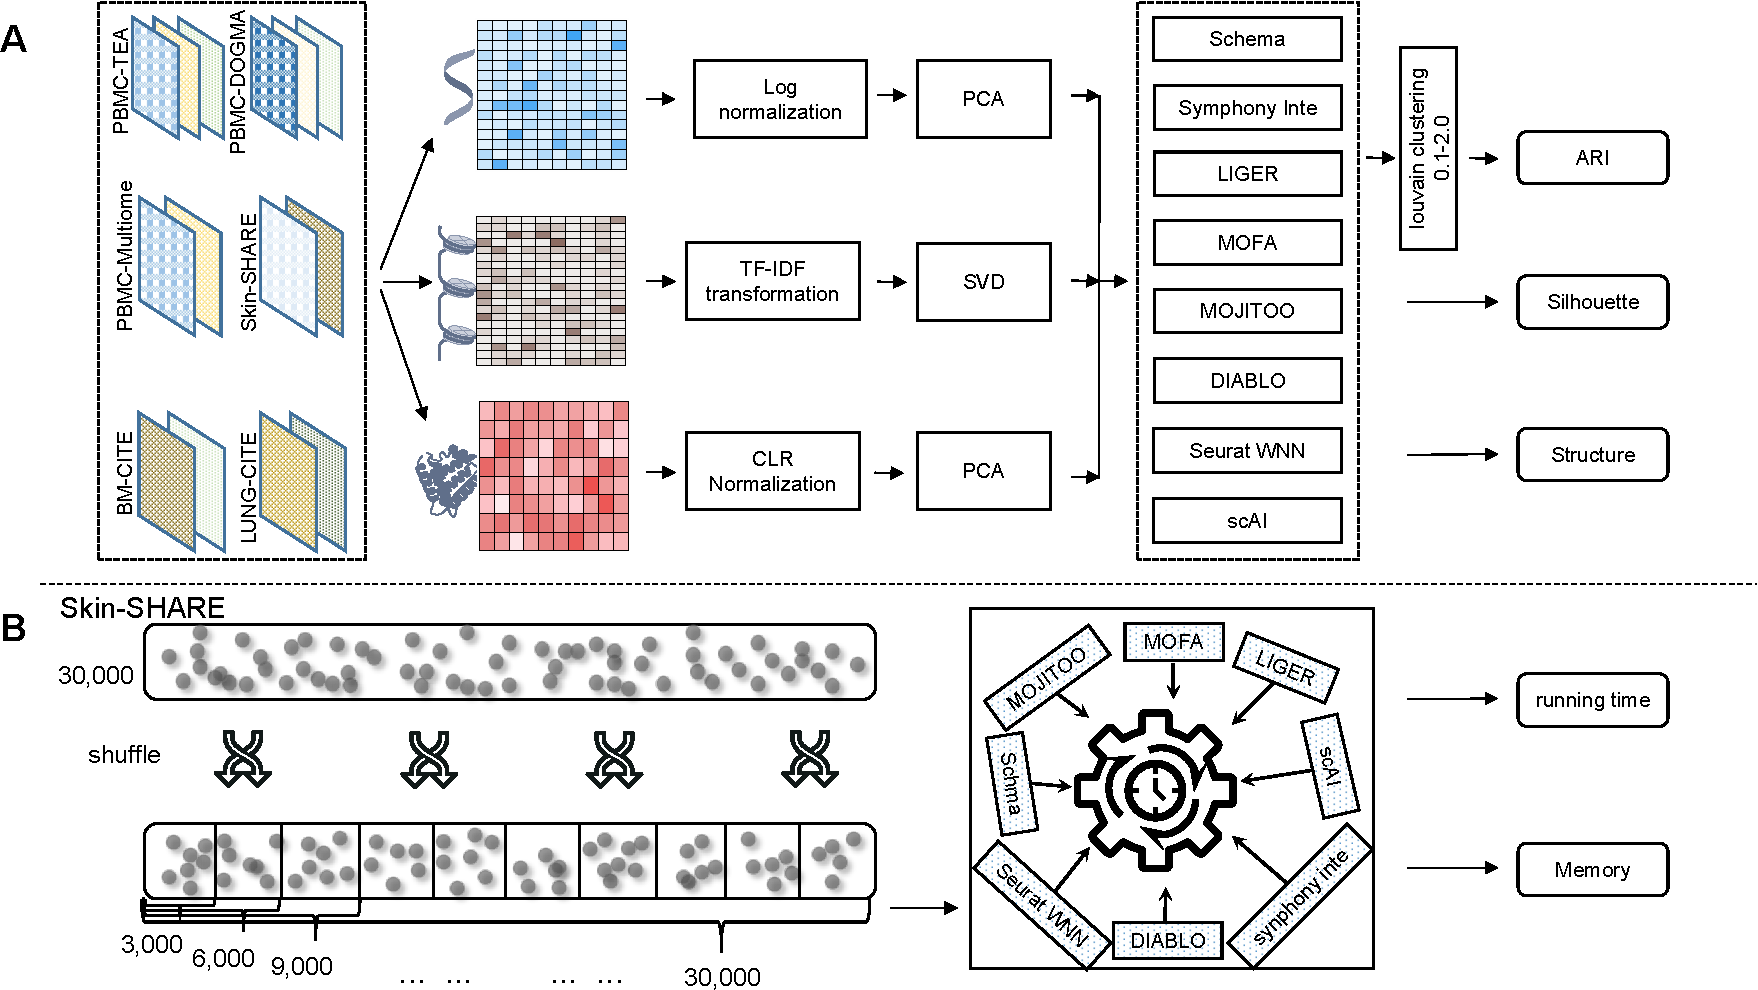
\includegraphics[width=0.95\textwidth]{evaluation_MOJITOO/fig}
	\vspace{0.1cm}
	\caption[MOJITOO evaluation workflow]{
	\textbf{MOJITOO evaluation workflow.} \textbf{A)} We input 6 single-cell multimodal datasets. Subsequently, we carry out pre-processing using standard pipelines from Seurat and Signac, followed by dimensional reduction. Harmony batch correction is applied to data \texttt{PMBC-TEA}, \texttt{BM-CITE}, and \texttt{LUNG-CITE} due to their batches. Integration methods are then executed to obtain the shared latent space. The evaluation of Adjusted Rand Index (ARI) requires clustering in the range from 0.1 to 2.0 with a step of 0.1. Silhouette score and Structure score are also utilized for benchmarking. \textbf{B)} We utilize the largest dataset, \texttt{Skin-SHARE}, to measure time consumption and memory usage for each competing method. Initially, we downsample the data from 30,000 cells to 3,000 with a step of 3,000 to obtain 10 different dataset sizes. Subsequently, all methods are executed to measure the time elapsed and peak memory usage.} 
	\label{fig:evaluation_MOJITOO}
\end{figure}

\begin{description} %%formula
	\item[Space Presevation] The high-dimensional space preserves of each dataset can be calculated as the Pearson correlation between all pairwise distances in the high-dimensional spaces and the corresponding distances in the original space~\citep{jain2021multimap}. For multimodal data, space-preserved scores can be obtained for each modality, and these individual scores are then averaged to derive the final space-preserved score.
	\item[Distance Accuracy]. 
  silhouette to latent space to evaluate the performance of these methods. For each data point $i\in C_i$, where $C_i$ is the label of the data point, we calculate the inner cluster mean distance:
\begin{equation}
  a(i) = \frac{1}{|C_i| - 1} \underset{j \in c_i, i\neq j}{\sum} d(i, j)
\end{equation}
Next, the smallest mean out cluster distance to data point $i$ is:
\begin{equation}
b(i) = \underset{k\neq i}{\min}\frac{1}{|C_k|}\underset{j\in c_k}{\sum} d(i,j)
\end{equation}
The solhoutte index is defined as:
\begin{equation}
s(i)=\frac{b(i)-a(i)}{\max\{a(i), b(i)\}}, -1\leq s(i) \leq 1
\end{equation}
where $d(i,j)$ is the distance of two cells under some specific latent space, here we considered both euclidean distance and cosine distance.

	\item[Clustering Accuracy] Clustering Accuracy measure the clustering accuracy compared to the true labels using different integrated embeddings. In comparing the clustering outcomes with labels from benchmarking datasets, we employed the adjusted rand index (ARI)\citep{hubert1985ARI}. This index assesses the similarity between two clustering results by accounting for the likelihood of randomly grouping elements. Specifically, given a dataset $D$ with $n$ cells, two partitions $ X = \{ X_{1}, X_{2}, \cdots X_{r} \} $ and $ Y = \{ Y_{1}, Y_{2}, \cdots, Y_{s} \} $ denoting different clustering results, the number of common cells for each cluster $i$ and $j$ can be written as $n_{ij} = X_{i} \cap Y_{j} |$, where $ i \in \{1, 2, \cdots, r \} $ and $ j \in \{1, 2, \cdots, s \} $. Then Adjusted Rand Index(ARI) is denoted as follows:
	\begin{equation}
		ARI = \frac{\sum_{ij} {n_{ij} \choose 2} - [ \sum_{i} {a_{i} \choose 2} \sum_{j} {b_{j} \choose 2 } ] / {n \choose 2}}{\frac{1}{2} [\sum_{i} {a_{i} \choose 2 } + \sum_{j} {b_{j} \choose 2}] - [\sum_{i} {a_{i} \choose 2} \sum_{j} {b_{j} \choose 2 } ] / {n \choose 2} }
	\end{equation}
	where $ a_{i} = \sum_{j=1}^{s} n_{ij} $ and $ b_{j} = \sum_{i=1}^{r} n_{ij} $ respectively. The ARI ranges from a minimum value of 0, denoting random agreement between two data clusterings, to a maximum value of 1, indicating identical clustering results.  To be fair, we perform Louvain clustering with varying resolution (parameter from 0.1 to 2.0 with step=0.1) to estimate the adjusted Rand index. 
	\item[Requirements of Memory and Running Time] We also compare the peak memory usage and running time to check the effectiveness of these methods. For this, we inspect the time and memory used in the largest datasets in our benchmark (SKIN-SHARE). To obtain curves, we down-sample the number of cells from 30,000 to 3,000.
\end{description}

% to validate improve the perfomance, ---> PBMC capture major cell types and subtype changings
%\subsection{Biological Insight}
%\label{MOJITOO:exp:bio}

\label{MOJITOO:exp:statistic}
% Nemenyi post-hoc test


\section{Results}
\label{MOJITOO:out}
In this section, we present the results generated by the single cell multimodal integration methods described in \sref{MOJITOO:exp}.

\subsection{Evaluation of multi-modal integration}
We present the benchmarking results using the data described in \sref{MOJITOO:exp:data} and the methods outlined in \sref{MOJITOO:exp:methods}. The evaluation is conducted based on the metrics outlined in \sref{MOJITOO:exp:metrics}.

\subsubsection{Benchmarking Structure Preseravtion}
First, we evaluate algorithms regarding their structure preservation, i.e. the average similarity between the Euclidean distances in the shared space and distances in the space of each modality\citep{jain2021multimap}. Results(\fref{fig:structure}) indicate the highest structure scores for MOJITOO (4 out of 6) followed by DIABLO (1 out of 6) and MOFA (1 out of 6). A ranking(\fref{fig:ranking}A) of the structure scores indicates MOJITOO as the best algorithm followed by DIABLO, MOFA, and Symph-Int. Interestingly, we observe that MOFA and Symph-Int tend to obtain higher structure scores for RNA and that MOJITOO and DIABLO have a lower variance of structure scores across modalities. This suggests that the MOJITOO and DIABLO shared space captures information of all individual modalities more uniformly than competing methods. The lower performance of Symphony integration compared to other CCA methods (MOJITOO and DIABLO) is explained by the fact it only considers CCs from the RNA space as integrated embedding.
\begin{figure}[!ht]
	\centering
	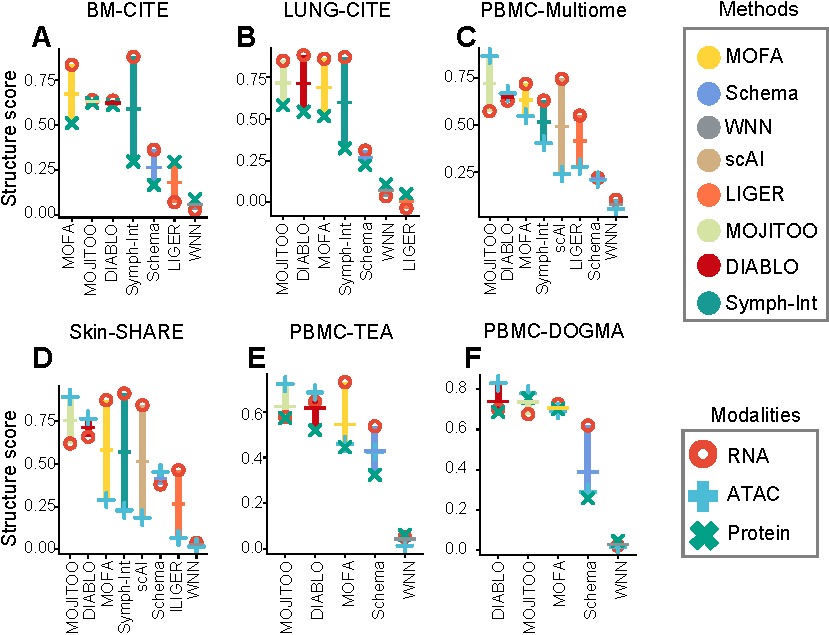
\includegraphics[width=0.95\textwidth]{structure/fig}
	\vspace{0.1cm}
	\caption[Evaluation of structure preservation for multi-modal integration methods.]{
	\textbf{Evaluation of structure preservation for multi-modal integration methods.}  We show the average (trace) and modality-specific structure scores (dots) (y-axis) versus methods (x-axis) for the six datasets.}
	\label{fig:structure}
\end{figure}

\subsubsection{Benchmarking Distance Accuracy}
Next, we make use of the cell types reported in the original manuscripts introducing the single-cell datasets as true labels for benchmarking. First, we use these labels to evaluate the silhouette scores by contrasting class labels with Euclidean distance matrices estimates on the shared space. Regarding silhouette(\fref{fig:silouette}), MOFA is best in four out of six datasets, while MOJITOO is best in the other two datasets. MOJITOO obtains second rank in four out of six datasets and is ranked second in the overall ranking(\fref{fig:ranking}). 
\begin{figure}[!ht]
	\centering
	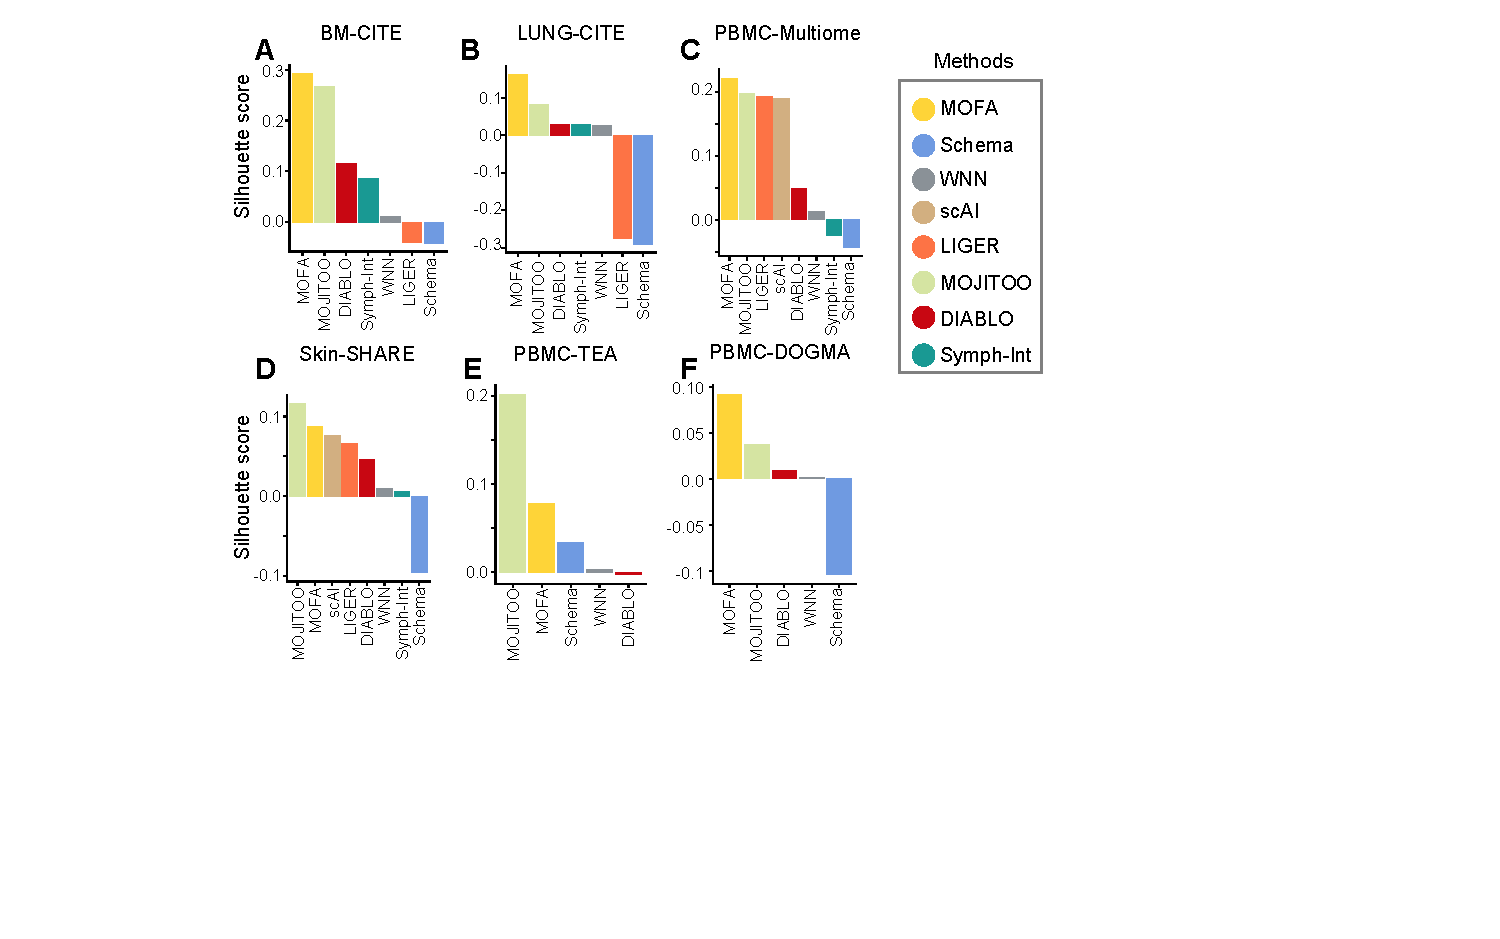
\includegraphics[width=0.95\textwidth]{silouette/fig}
	\vspace{0.1cm}
	\caption[Evaluation of distance accuracy for multi-modal integration methods.]{
        \textbf{Evaluation of distance accuracy for multi-modal integration methods.} Barplots showing silhouette score (y-axis) versus methods (x-axis) for six benchmark datasets. }
	\label{fig:silouette}
\end{figure}

\subsubsection{Benchmarking Clustering Accuracy}
we perform Louvain clustering at distinct resolutions (0.1–2.0) on the shared latent space. We then measure the agreement of clustering results with labels using the Adjusted Rand Index (ARI)(\fref{fig:ari}). WNN and Symphony have the highest ARI in two datasets each, while DIABLO and MOJITOO have the highest values in one dataset each. MOJITOO has a higher rank than two in all datasets and has the highest overall rank followed by WNN and DIABLO\fref{fig:ranking}. Moreover, we also perform a sensitivity analysis on MOJITOO to inspect if the dimension of the original PCA/LSI space has an impact on its performance \afref{fig:Input_Dimensions}. We observe that if 50 or more components are used, MOJITOO obtains similar clustering and structure preservation scores. 
\begin{figure}[!ht]
	\centering
	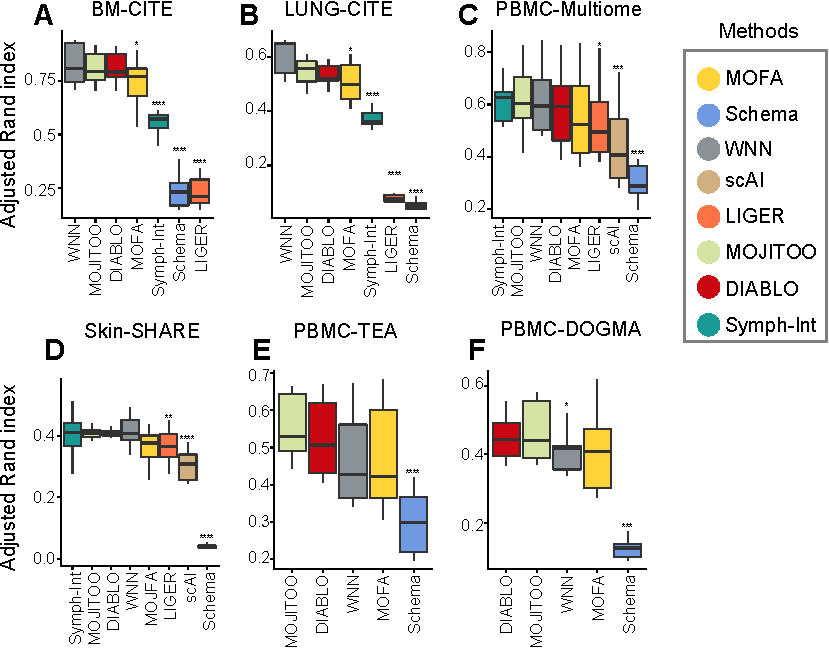
\includegraphics[width=0.95\textwidth]{ari/fig}
	\vspace{0.1cm}
	\caption[Evaluation of clustering accuracy for multi-modal integration methods.]{
	\textbf{Evaluation of clustering accuracy for multi-modal integration methods.} Boxplots showing ARI scores (y-axis) versus methods (x-axis) for distinct clustering solutions for all six data sets. Asterisks indicate P-values of $<$0.05(*), $<$0.01(**), $<$0.001(***), $<$0.0001(****) obtained via t-test comparing the ARI values of MOJITOO versus other methods. }
	\label{fig:ari}
\end{figure}

\begin{figure}[!ht]
	\centering
	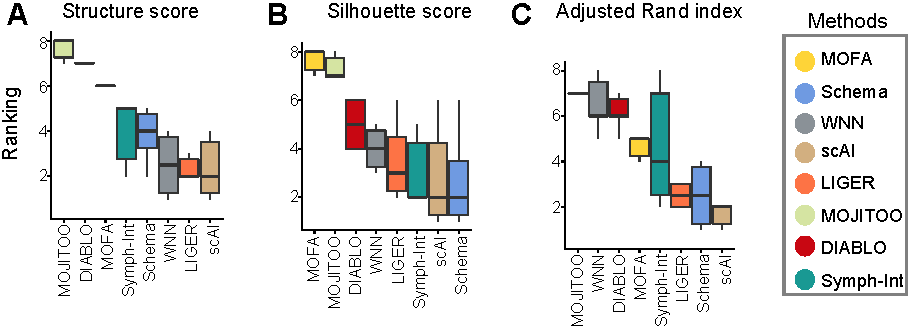
\includegraphics[width=0.95\textwidth]{ranking/fig}
	\vspace{0.1cm}
	\caption[Evaluation of ranking for multi-modal integration methods.]{\textbf{Evaluation of ranking for multi-modal integration methods.} \textbf{A)} Boxplots showing the combined structure score ranking of the method over all datasets, where the highest rank indicates the best performer. \textbf{B)} Boxplots showing the combined silhouette score ranking of the method over all datasets, where the highest rank indicates the best performer. \textbf{C)} Boxplots showing the combined ARI score ranking of the method over all datasets, where the highest rank indicates the best performer.}
	\label{fig:ranking}
\end{figure}

\subsubsection{Benchmarking Requirements of Memory and Time}
We next evaluated the memory usage and running time consumption of single-cell integration methods, as illustrated in \fref{fig:time_memory}. Overall, MOJITOO demonstrated the lowest time consumption (\fref{fig:time_memory}B and \atref{tab:memory}) and minimal memory requirements (\fref{fig:time_memory}B and \atref{tab:time}). In the largest dataset with 30,000 cells, MOJITOO exhibited the fastest performance, completing the analysis in only 2.5 minutes and utilizing 6.4 GB of memory. The low memory requirements suggest that MOJITOO can even run efficiently on commonly available laptops for large datasets with over 100,000 cells. These results indicate that MOJITOO exhibits excellent scalability.
\begin{figure}[!ht]
	\centering
	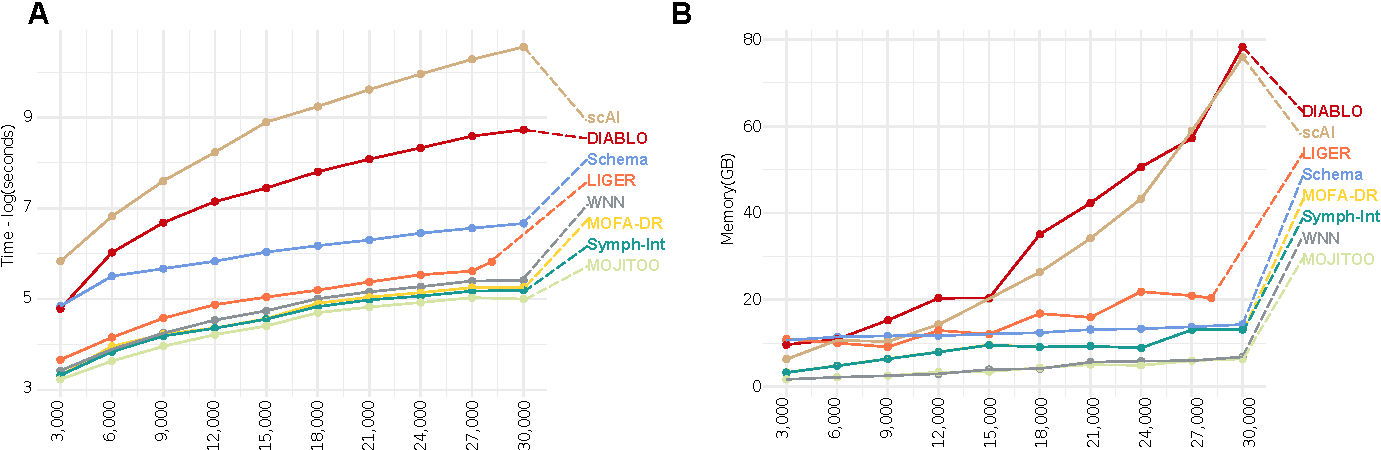
\includegraphics[width=0.95\textwidth]{time_memory/fig}
	\vspace{0.1cm}
	\caption[Evaluation of time and memory consumption for multi-modal integration methods.]{\textbf{Evaluation of time and memory consumption for multi-modal integration methods.} Time and memory consumption on the Skin-SHARE. (A) Line plots showing elapsed time (log of seconds) for each method (y-axis). (B) Line plots showing peak memory (Gigabytes) required by each method (y-axis). In both A–B, the x-axis shows the number of cells used (randomly sampled) from the \texttt{Skin-SHARE} data}
	\label{fig:time_memory}
\end{figure}

\subsection{Evaluation of PBMC data}
Examples of low dimensional embeddings obtained by distinct integration methods with the PBMC-Multiome dataset are provided in 


Additionally, we explore the use of the dimensions of the latent space ($Z$) as factors for interpreting the PBMC multiome data. We denote the latent features as canonical components (CC). As shown in \fref{fig:CC_UMAP}, positive or negative values for the top CCs discern well all major cell types (Fig.~\ref{fig:CC_UMAP}). High values of CC1 are associated to myeloid cells (CD14+ and CD16+ monocytes and dendritic cells), while negative values are associated to T and NK cells (\fref{fig:CC_UMAP}A). CC2 values discern B cell and plasmacytoid dendritic cells (pDC) from other cells, while CC3 differentiates B cells from pDCs (\fref{fig:CC_UMAP}B-C). Further CCs capture subtle changes between major cell sub-types (Fig.~\ref{fig:CC_UMAP}D-E). CC4 and CC5 capture changes between naive T cells and active T CD8 and active T CD4 cells respectively, while CC5 captures differences between naive monocytes (CD14+) and activated monocytes (CD16+). Other smaller cell types (dendritic cells, platelets, double negative T cells and pre-B and progenitor B cells) can be characterized with further CCs (Supplementary Fig.~5). We also evaluated CCs with low correlation, which were considered as noise by MOJITOO (Supplementary Fig. 6). We observe that these CCs have high scores for a few cells and low concordance across modalities. This supports their low biological relevance.


Next, we explore the $U$ matrices, which provide values associating molecular features with the latent dimensions (CCs). Indeed, the expression of genes with high CC1 values includes monocyte genes such as LYN and FCN1, while negative CC1 values are associated to T cell genes BCL11B and IL7R (\fref{fig:CC_Genes}A). Similarly, we observe that top-ranked peaks with high or low CC1 scores have monocyte or T cell-specific open chromatin. These include regions close to the T cell gene BCL11B (\fref{fig:CC_Peaks}A). High CC2 values are associated with B cell genes IGHM and BCL11A, while low CC1 genes (BCBL11B and IL32) are associated with T cells (\fref{fig:CC_Genes}B). As before, we observe cell-specific open chromatin patterns on top-ranked ATAC-seq peaks associated with high and low CC2 values(\fref{fig:CC_Peaks}B). Altogether, these results indicate that MOJITOO CCs can be used to capture major cell types of peripheral blood cells as well as to detect modality-specific molecular features associated to these.


\fref{fig:pbmc_multiome_umap}.
\begin{figure}[!ht]
	\centering
	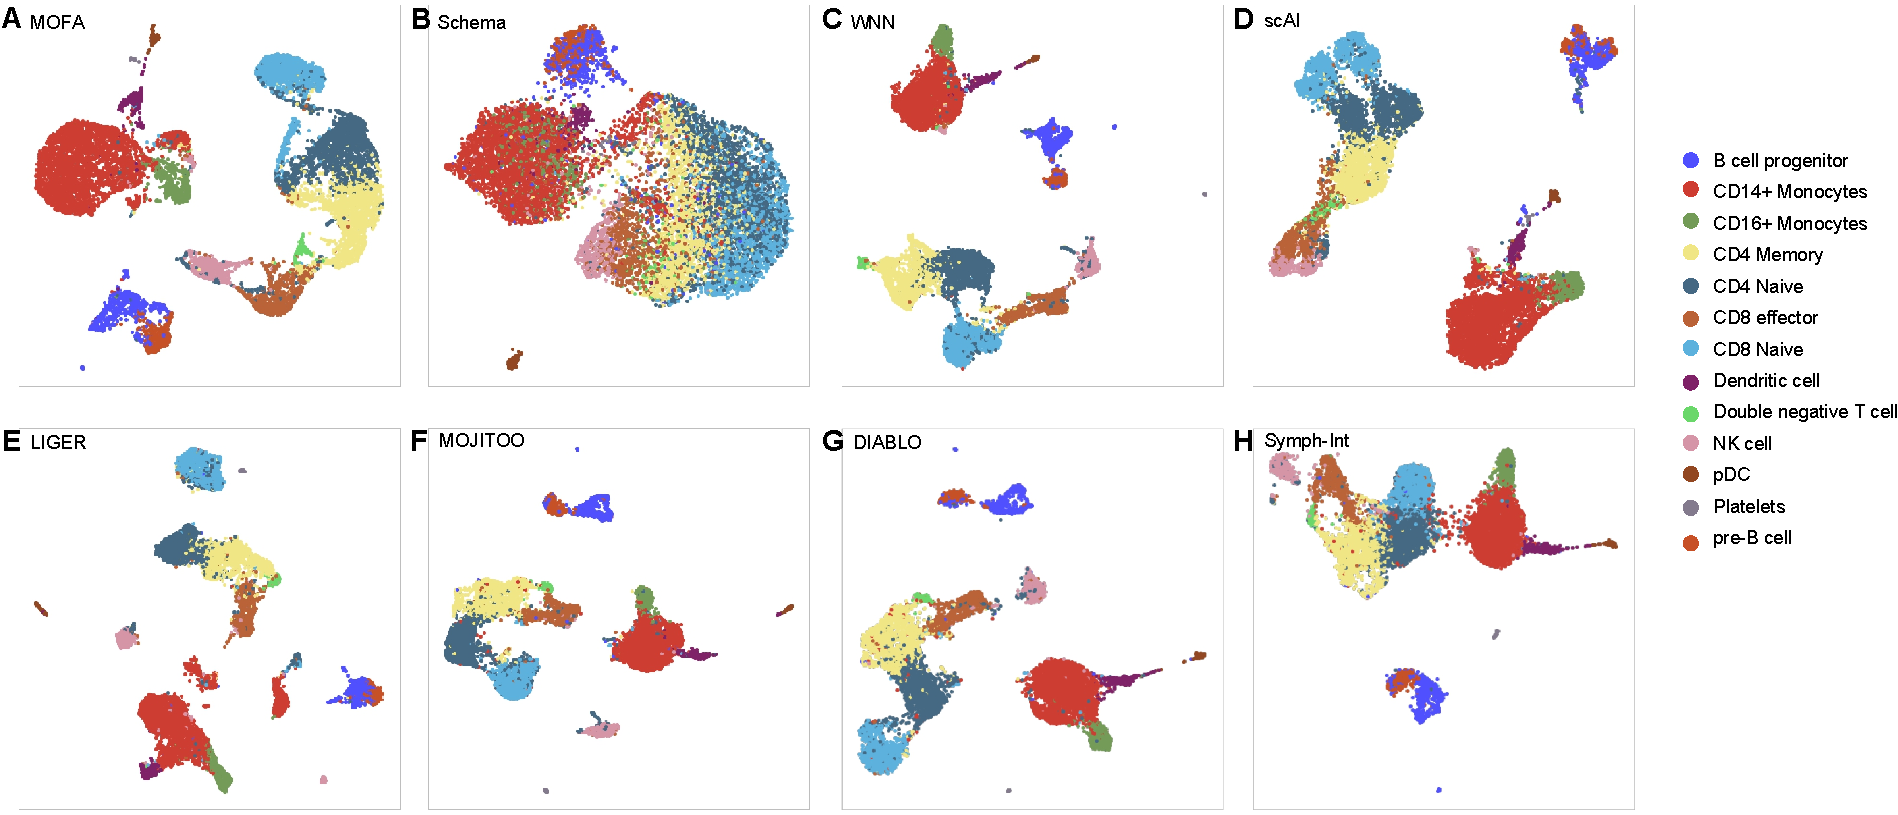
\includegraphics[width=0.95\textwidth]{pbmc_multiome_umap/fig}
	\vspace{0.1cm}
	\caption[UMAP of multiome PBMC comparison for different multi-modal integration methods.]{\textbf{UMAP of multiome \texttt{PBMC-multiome} comparison for different multi-modal integration methods.}UMAPs showing cell type distribution derived from integration methods on \texttt{PBMC-multiome} dataset. }
	\label{fig:pbmc_multiome_umap}
\end{figure}

\begin{figure}[!ht]
	\centering
	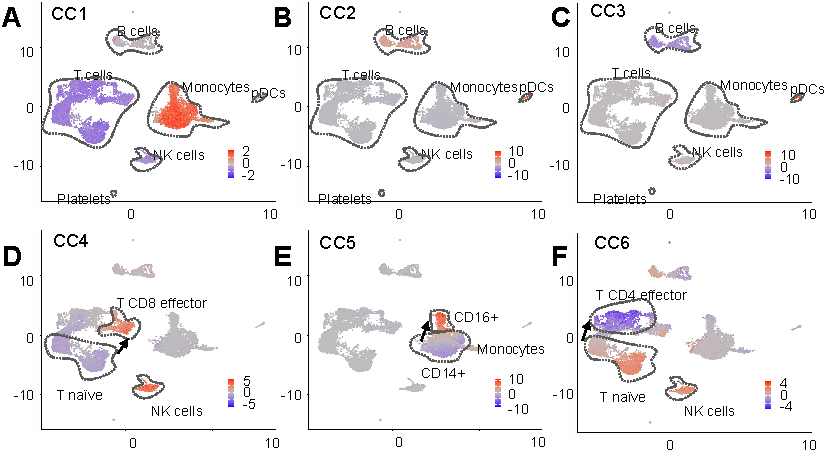
\includegraphics[width=0.95\textwidth]{CC_UMAP/fig}
	\vspace{0.1cm}
	\caption[CCs in the UMAP.]{\textbf{CCs in the UMAP.} (A–F) UMAP with the scores of CC1 to CC6. We highlight major cell types (or sub-types) associated to positive or negative CC scores and arrows indicate directions associated to the activation of particular immune cells}
	\label{fig:CC_UMAP}
\end{figure}


\begin{figure}[!ht]
	\centering
	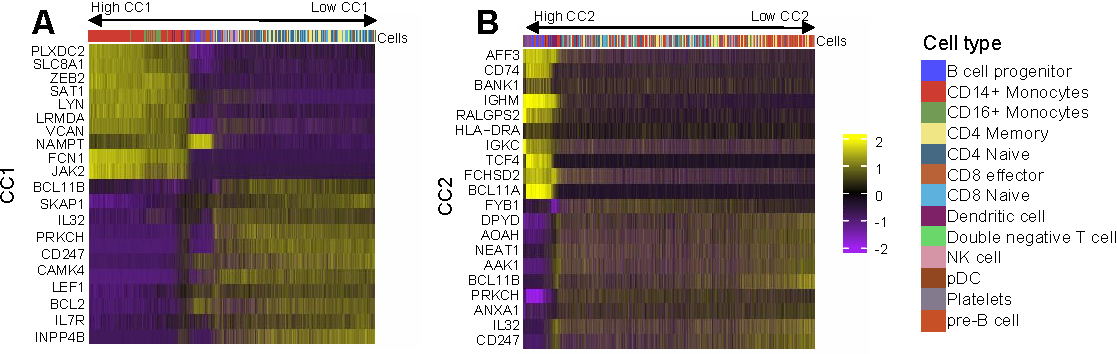
\includegraphics[width=0.95\textwidth]{CC_Genes/fig}
	\vspace{0.1cm}
	\caption[Heatmaps of top 10 positive and negative genes select by CC1 and CC2.]{\textbf{Heatmaps of top 10 positive and negative genes select by CC1 and CC2.} \textbf{A)} Heatmap with scores for the top 10 positive and negative genes for CC1 (y-axis) versus cells (x-axis). Cells are ordered by CC1 scores (high to low). \textbf{B)} showing the heatmap of top genes for CC2}
	\label{fig:CC_Genes}
\end{figure}


\begin{figure}[!ht]
	\centering
	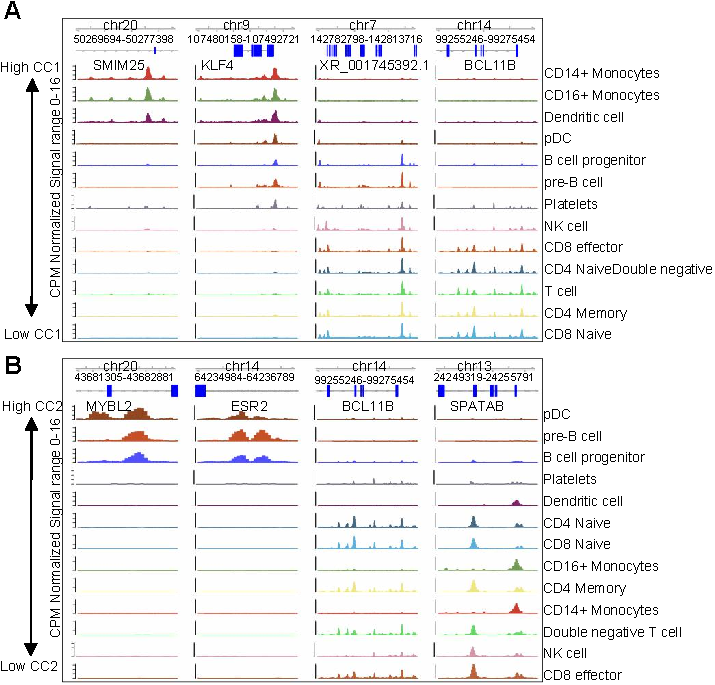
\includegraphics[width=0.95\textwidth]{CC_Peaks/fig}
	\vspace{0.1cm}
	\caption[Genome browser tracks of top 2 positive and negative peaks for CC1 and CC2.]{ \textbf{A)} Genome browser tracks with top 2 positive and negative peaks for CC1. Tracks correspond to normalized cell-specific pseudo bulk ATAC-seq profiles generated by deeptools \citep{ramirez2016deeptools2}. Cell-specific tracks are ordered by CC1 score (high to low). \textbf{B)} showing the genome browser of top peaks for CC2.}
	\label{fig:CC_Peaks}
\end{figure}

\section{Statistical methods}
For comparisons involving multiple methods and datasets, we employed the non-parametric Friedman test with the Nemenyi post-hoc test (Demšar, 2006). The Friedman test(Friedman, 1937, 1940) was utilized to compare the average ranks of the methods across all datasets. The null hypothesis assumes that all the methods are equivalent, and their ranks are equal. We utilized the friedmanTest function from the R package PMCMRplus to conduct the Friedman rank sum test. If the null hypothesis was rejected, indicating that at least one method is significantly different from the others, we proceeded with the Nemenyi post-hoc test (Nemenyi, 1963) to compare all pairs. Therefore, to compare k methods, a total of $k(k-1)/2$ hypotheses were tested, and this was accomplished using the frdAllPairsNemenyiTest function from the R package PMCMRplus.

\section{Discussion}

In this chapter, we described the experimental framework to evaluate our computational method and next present the benchmarking results.

A comprehensive analysis with six bi-modal and tri-modal multimodal datasets indicates that MOJITOO has the best performance regarding the preservation of the structures across modalities and the recovery of clusters, while it is ranked second regarding distance representation. Moreover, MOJITOO has the lowest time and memory requirements requiring 2.5 min and 6.4 GB in the largest dataset with 30.000 cells. WNN, which is the standard method for integration in Seurat, performed well on the clustering problem (2nd after MOJITOO) and had a low computational time, but had a poor performance in the structure preservation and silhouette scores. Moreover, WNN, which outputs a distance matrix on the shared space, does not provide latent features as MOJITOO, DIABLO or MOFA. MOFA performed well on distance representation, but was ranked fourth in the clustering problem and third at structure preservation score. DIABLO, which is also based in CCA, had an good predictive performance (2nd for structure preservation and 3rd in clustering and distance preservation), but had an a poor computational performance being the 2nd slowest method.

An interesting result is the fact the structure preservation scores are more uniform across modalities for CCA-based methods MOJITOO and DIABLO, while runner-up methods (MOFA) obtained highest scores for the RNA modality. This is possibly rooted on the analytical frameworks of these methods. CCA analysis explicitly finds canonical vectors with high correlation across modalities, while matrix factorization methods (MOFA) do not explicitly guarantee factors are uniformly well represented across modalities. Of note, the CCA approach explored in Symphony was also biased toward structure preservation in RNA, due to the fact it only use RNA canonical vectors as a final latent representation. 

